%%%------------------------------------------------------------------------------------------------------------
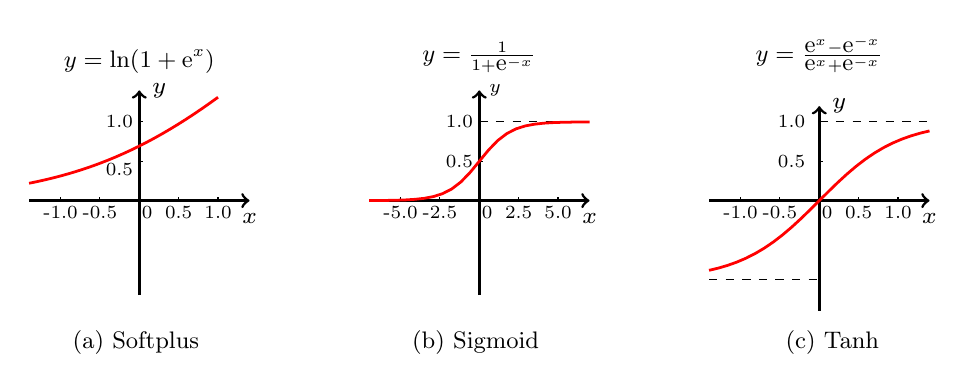
\begin{tikzpicture}
\tikzstyle{every node}=[scale=1.2]
\begin{scope}
\draw[->, line width=1pt](-1.4,0)--(1.4,0)node[left,below,font=\scriptsize]{$x$};
\draw[->, line width=1pt](0,-1.2)--(0,1.4)node[right,font=\scriptsize]{$y$};
\foreach \x in {-1.0,-0.5,0.5,1.0}{\draw(\x,0)--(\x,0.05)node[below,outer sep=2pt,font=\scriptsize,scale=0.8]at(\x,0.1){\x};}
\node[below,outer sep=2pt,font=\scriptsize,scale=0.8]at(0.1,0.1){0};
 \foreach \y in {1.0,0.5}{\draw(0,\y)--(0.05,\y)node[left,outer sep=2pt,font=\scriptsize,scale=0.8]at(0.1,\y){};}
\node[left,outer sep=2pt,font=\scriptsize,scale=0.8]at(0.1,0.4){0.5};
\node[left,outer sep=2pt,font=\scriptsize,scale=0.8]at(0.1,1.0){1.0};
\draw[color=red ,domain=-1.4:1.0, line width=1pt]plot(\x,{ln(1+(exp(\x))});
\node[black,anchor=south,scale=0.8] at (0,1.5) {\small $y = \ln(1+{\textrm e}^x)$};
\node [anchor=south east,inner sep=1pt,scale=0.8] (labela) at (0.8,-2) {\small{(a) Softplus}};
\end{scope}

%%%------------------------------------------------------------------------------------------------------------
\begin{scope}[xshift=1.7in]

\draw[->, line width=1pt](-1.4,0)--(1.4,0)node[left,below,font=\scriptsize]{$x$};
\draw[->, line width=1pt](0,-1.2)--(0,1.4)node[right,font=\scriptsize,scale=0.8]{$y$};
\draw[dashed](0,1)--(1.4,1);
\foreach \x in {-1,-0.5,0.5,1}{\draw(\x,0)--(\x,0.05)node[below,outer sep=2pt,font=\scriptsize,scale=0.8]at(\x,0.1){
      \pgfmathparse{(\x)*5}
      \pgfmathresult};}
\node[below,outer sep=2pt,font=\scriptsize,scale=0.8]at(0.1,0.1){0};
\foreach \y in {0.5,1.0}{\draw(0,\y)--(0.05,\y)node[left,outer sep=2pt,font=\scriptsize,scale=0.8]at(0.1,\y){\y};}
\draw[color=red,domain=-1.4:1.4, line width=1pt]plot(\x,{1/(1+(exp(-5*\x)))});
\node[black,anchor=south,scale=0.8] at (0,1.5) {\small $y = \frac{1}{1+{\textrm {e}}^{-x}}$};
\node [anchor=south east,inner sep=1pt,scale=0.8] (labelb) at (0.8,-2) {\small{(b) Sigmoid}};
\end{scope}
%%%------------------------------------------------------------------------------------------------------------

\begin{scope}[xshift=3.4in]
 \draw[->, line width=1pt](-1.4,0)--(1.4,0)node[left,below,font=\scriptsize]{$x$};
        \draw[->, line width=1pt](0,-1.4)--(0,1.2)node[right,font=\scriptsize]{$y$};
        \draw[dashed](0,1)--(1.4,1);
        \draw[dashed](-1.4,-1)--(0,-1);
        \foreach \x in {-1.0,-0.5,0.5,1.0}{\draw(\x,0)--(\x,0.05)node[below,outer sep=2pt,font=\scriptsize,scale=0.8]at(\x,0.1){\x};}
        \node[below,outer sep=2pt,font=\scriptsize,scale=0.8]at(0.1,0.1){0};
        \foreach \y in {0.5,1.0}{\draw(0,\y)--(0.05,\y)node[left,outer sep=2pt,font=\scriptsize,scale=0.8]at(0,\y){\y};}
        \draw[color=red ,domain=-1.4:1.4, line width=1pt]plot(\x,{tanh(\x)});
        \node[black,anchor=south,scale=0.8] at (0,1.5) {\small $y = \frac{{\textrm e}^{x}-{\textrm e}^{-x}}{\textrm{e}^{x}+{\textrm e}^{-x}}$};
\node [anchor=south east,inner sep=1pt,scale=0.8] (labelc) at (0.8,-2) {\small{(c) Tanh}};
\end{scope}
\end{tikzpicture}
%%%------------------------------------------------------------------------------------------------------------